Our challenge for this app is to find the best availabe deals for the items in a given shoping list.
We have decided to split the solution into three different parts: The front end, the back end and the database.
Our front end will take a shoping list from the user, and the back end will find the best possible deal and give it back to the user.
The best possible deal might be not be the cheapest item but it might be a deal that saves the user travel distance time at a slightly higher item price.
The database is going to store various types of user data like login information, previous groceries list, etc.

\begin{figure}
    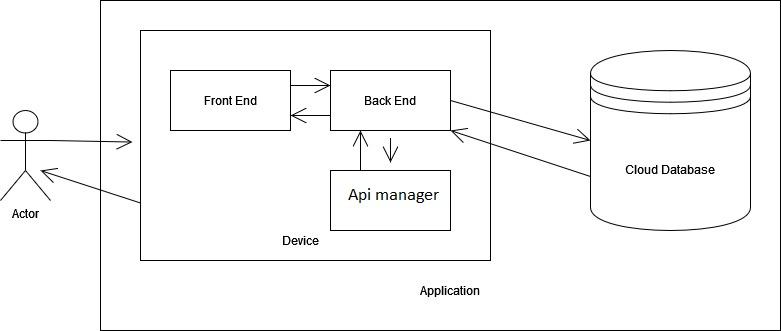
\includegraphics{images/system diagram.jpg}
    \caption{A high level overview of the system}
\end{figure}
